\documentclass[a4paper]{article}
% Kodowanie latain 2
%\usepackage[latin2]{inputenc}
\usepackage[T1]{fontenc}
% Można też użyć UTF-8
\usepackage[utf8]{inputenc}
% Język
\usepackage[polish]{babel}
% \usepackage[english]{babel}
\usepackage{tikz}
% Rózne przydatne paczki:
% - znaczki matematyczne
\usepackage{amsmath, amsfonts}
% - wcięcie na początku pierwszego akapitu
%\usepackage{indentfirst}
% - komenda \url 
\usepackage{hyperref}
\usepackage{graphicx}
\graphicspath{ {.} }
% - szersza strona
\usepackage[nofoot,hdivide={2cm,*,2cm},vdivide={2cm,*,2cm}]{geometry}
\frenchspacing
% - brak numerów stron
\pagestyle{empty}

% dane autora
\author{Weronika Domczewska}
\title{sprawdzian\LaTeX}
\date{\today}

% początek dokumentu
\begin{document}

\noindent \large Weronika Domczewska 323621 \hfill 30.11.2020
\medskip

\begin{center}
{\noindent \bf \large Sprawozdanie poprawkowe ze sprawdzianu 1}
\end{center}

\subsection*{Zadanie 1}

\begin{itemize}
    \item $\rho \frac{Du}{Dt} = (\rho \frac{\partial u}{\partial t} + \textbf u \cdot \nabla \textbf u) =  -\nabla \bar{p} + \nabla \cdot \{\mu (\nabla \textbf{u} + \nabla \textbf{u})^ T - \frac{2}{3} (\nabla \cdot u) \textbf{I}\} + \rho \sf g$ 
\end{itemize}

\begin{itemize}
    \item $\tilde{f} (\xi) = \int_{-\infty}^{\infty} f(x) e^{-2\pi i x \xi} dx$
\end{itemize}

\begin{itemize}
    \item $\mathbb{P}(\hat{X}_n - z_1 - _\frac{\alpha}{2} \frac{\sigma}{\sqrt{n}} \leq \mathbb{E}X \leq \hat{X}_n - z_1 - _\frac{\alpha}{2} \frac{\sigma}{\sqrt{n}}) \approx 1 - \alpha$
\end{itemize}

\begin{itemize}
    \item $\begin{bmatrix}
        1 && 2\\
        3 && 4 
    \end{bmatrix} \otimes 
    \begin{bmatrix}
        0 && 5\\
        6 && 7
    \end{bmatrix} = 
    \begin{bmatrix}
        1 
        \begin{bmatrix}
            0 && 5\\
            6 && 7
        \end{bmatrix} 
        2
        \begin{bmatrix}
            0 && 5\\
            6 && 7
        \end{bmatrix} \\
        3
        \begin{bmatrix}
            0 && 5\\
            6 && 7
        \end{bmatrix} 
        4
        \begin{bmatrix}
            0 && 5\\
            6 && 7
        \end{bmatrix}
    \end{bmatrix} = 
    \begin{bmatrix}
        0 && 5 && 0 && 10\\
        6 && 7 && 12 && 24\\
        0 && 15 && 0 && 20\\
        18 && 21 && 24 && 28  
    \end{bmatrix}$
\end{itemize}

\subsection*{Zadanie 2}
1. 

\begin{center}
    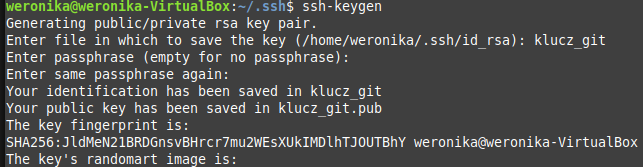
\includegraphics[scale=0.5]{2_1.png}

    \noindent Analogicznie wygenerowałam klucz do serwera.

\end{center}

\noindent 2.

\begin{center}
    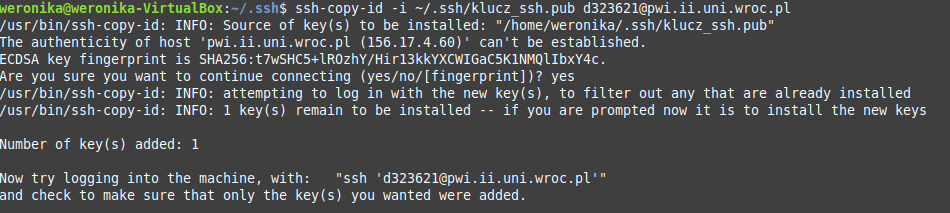
\includegraphics[scale=0.5]{2_2.png}

    \noindent Przełącznik -i (identity file) zapewnia dodanie jedynie wybranego przez nas klucza.

\end{center}

\noindent 3.

\begin{center}
    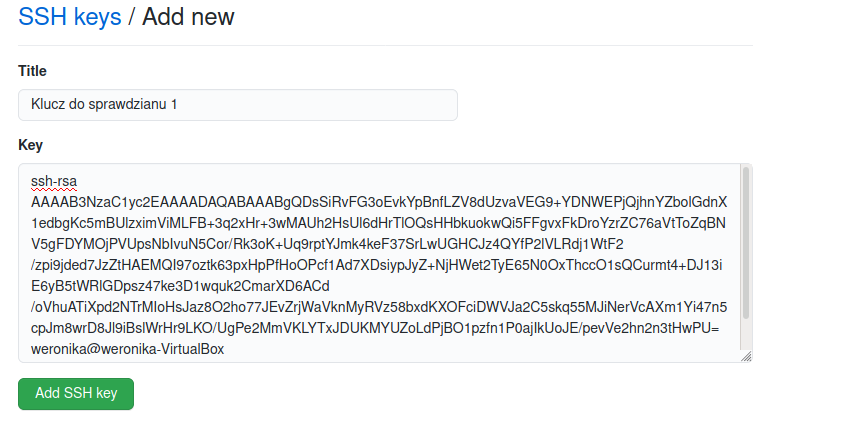
\includegraphics[scale=0.4]{2_3.png}
    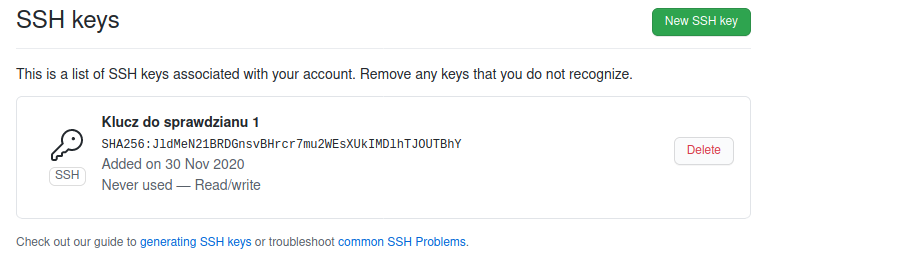
\includegraphics[scale=0.4]{2_31.png}

\end{center}

\noindent 4.

\begin{center}
    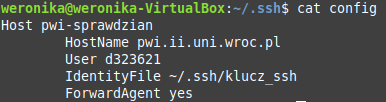
\includegraphics[scale=0.4]{2_4.png}
\end{center}

\noindent 5. Klucz lokalny przekierowuję poprzez dodanie do pliku konfiguracyjnego opcji \\ \verb+ForwardAgent yes+

\begin{center}
    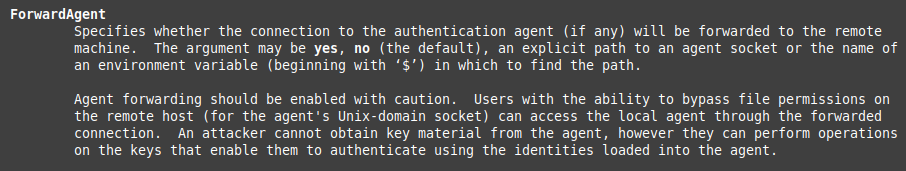
\includegraphics[scale=0.4]{2_5.png}
\end{center}

\subsection*{Zadanie 3}
1. 

\begin{center}
    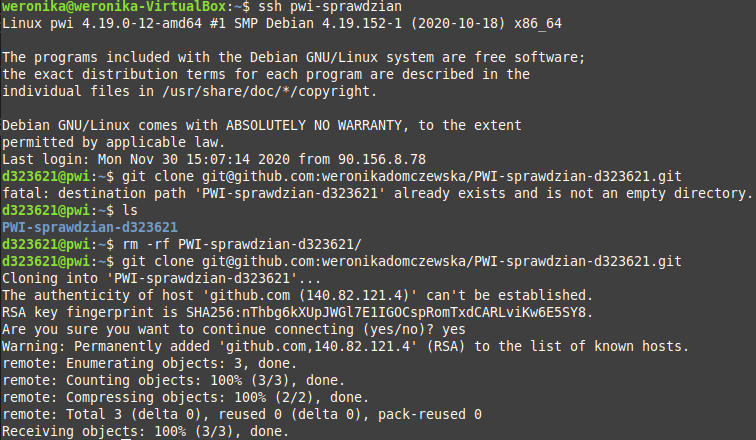
\includegraphics[scale=0.4]{3_1.png}
\end{center}

\noindent Generowanie kolejnego klucza na zdalnym komputerze jest "brzydkie", ponieważ klucz jest jak nasz podpis - pozwala nas zidentyfikować w jednoznaczny sposób. Kiedy generujemy drugi klucz, utrudniamy identyfikację.

\noindent 2. 

\noindent Pobrałam plik przy pomocy \verb+wget http://www.ii.uni.wroc.pl/~lisu/zadanie.tar.gz+

\noindent Wypakowałam plik przy pomocy polecenia \verb+tar -xvf zadanie.tar.gz+

\noindent Znaczenie przełączników: \\
\verb+-x+ -  wypakuj plik \\
\verb+-v+ - pokaż postęp wypakowywania (informacje o wypakowanych plikach) \\
\verb+-f+ - nazwa archiwum do wypakowania \\

\noindent Skomitowałam wszystko przy pomocy poleceń \verb+git add .+ oraz \verb+git commit+

\newpage

\noindent 3.

\begin{center}
    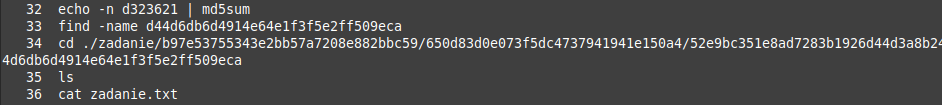
\includegraphics[scale=0.4]{3_3.png}
\end{center}

\noindent Znaczenie przełączników w \verb+echo+: \\
\noindent \verb+echo+ - wypisz na konsolę
\noindent \verb+-n+ - nie dodawaj na koniec znaku nowej linii \\
\noindent \verb+|+ - przekieruj output \verb+echo+ do następnego programu \\
\noindent \verb+md5sum+ - program do wyznaczania funkcji skrótu MD5 ze stringa \\

\noindent Znaczenie przełączników w \verb+find+: \\
\noindent \verb+-name+ - szukaj w folderze po nazwie

Zadania z pliku \verb+zadanie.txt+:

\begin{center}
    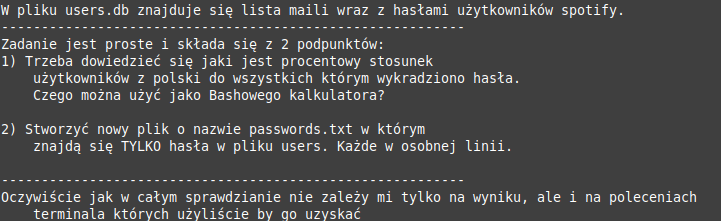
\includegraphics[scale=0.4]{zadanie.png}
\end{center}

\noindent Podpunkt 1 \\
\noindent Jako kalkulatora używam \verb+python3+.

\begin{center}
    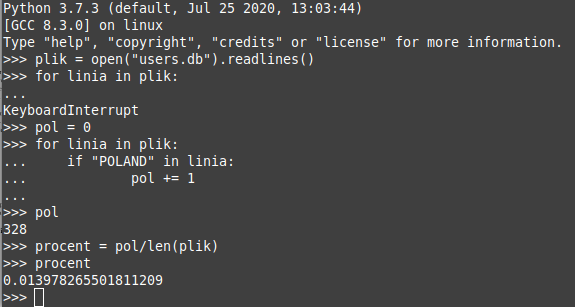
\includegraphics[scale=0.4]{zadanie1.png}
\end{center}
Użytkownicy z Polski stanowili około 1.4\% użytkowników \\

\noindent Podpunkt 2

\begin{center}
    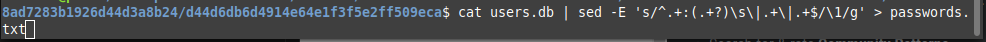
\includegraphics[scale=0.4]{zadanie2.png}
\end{center}

\noindent Znaczenie komend: \\
\noindent \verb+cat+ - wypisz zawartość pliku \\
\noindent \verb+sed+ - program do dokonywania zmian w tekście \\
\noindent \verb+-E+ - użyj rozszerzonych instrukcji RE \\
\noindent \verb+s+ - zamień \\
\noindent wyrażenie regularne - od początku do końca linii znajdź cokolwiek co występuje przynajmniej raz, następnie dwukropek, potem hasło złożone z czegokolwiek, co występuje przynajmniej raz (? - wyszukujemy do pierwszego wystąpienia znaku białego), następnie szukamy pipe, po nim cokolwiek, pipe i cokolwiek do końca linii \\
\noindent \verb+\1+ - zastąp całą linię znalezionym hasłem \\
\noindent \verb+g+ - zastąp w całym pliku \\
\noindent \verb+> passwords.txt+ - przekieruj wynik do pliku passwords.txt \\

\newpage
\textbf Bibliografia:
\begin{itemize}
    \item \url{https://www.digitalocean.com/community/tutorials/how-to-configure-custom-connection-options-for-your-ssh-client}
    \item \url{https://linuxize.com/post/using-the-ssh-config-file/}
    \item \url{https://oeis.org/wiki/List_of_LaTeX_mathematical_symbols}
    \item \url{https://regexr.com/}
    \item \url{https://www.geeksforgeeks.org/sed-command-in-linux-unix-with-examples/}

\end{itemize}

\end{document}